\section{Vergleich beider Systeme} \label{sec:systemvergleich}

Der Vergleich des Systemverhaltens des nichtlinearen (\autoref{fig:Bild2}) und des linearen Systems (\autoref{fig:Bild3}) wird in der stabilen Ruhelage durchgeführt, da hierzu keine Reglerstruktur benötigt wird. Der Vergleich wird auf Grundlage der Winkellage durchgeführt. Für den direkten Vergleich wird zu jedem Zeitpunkt ein radialer Winkel Pi zu dem Winkel $\varphi$ des linearen Systems addiert. Als Testsignal wird ein Einheitssprung nach 0.5s mit der Amplitude Eins eingeprägt.

\begin{figure}[H]
   \centering
   \fbox{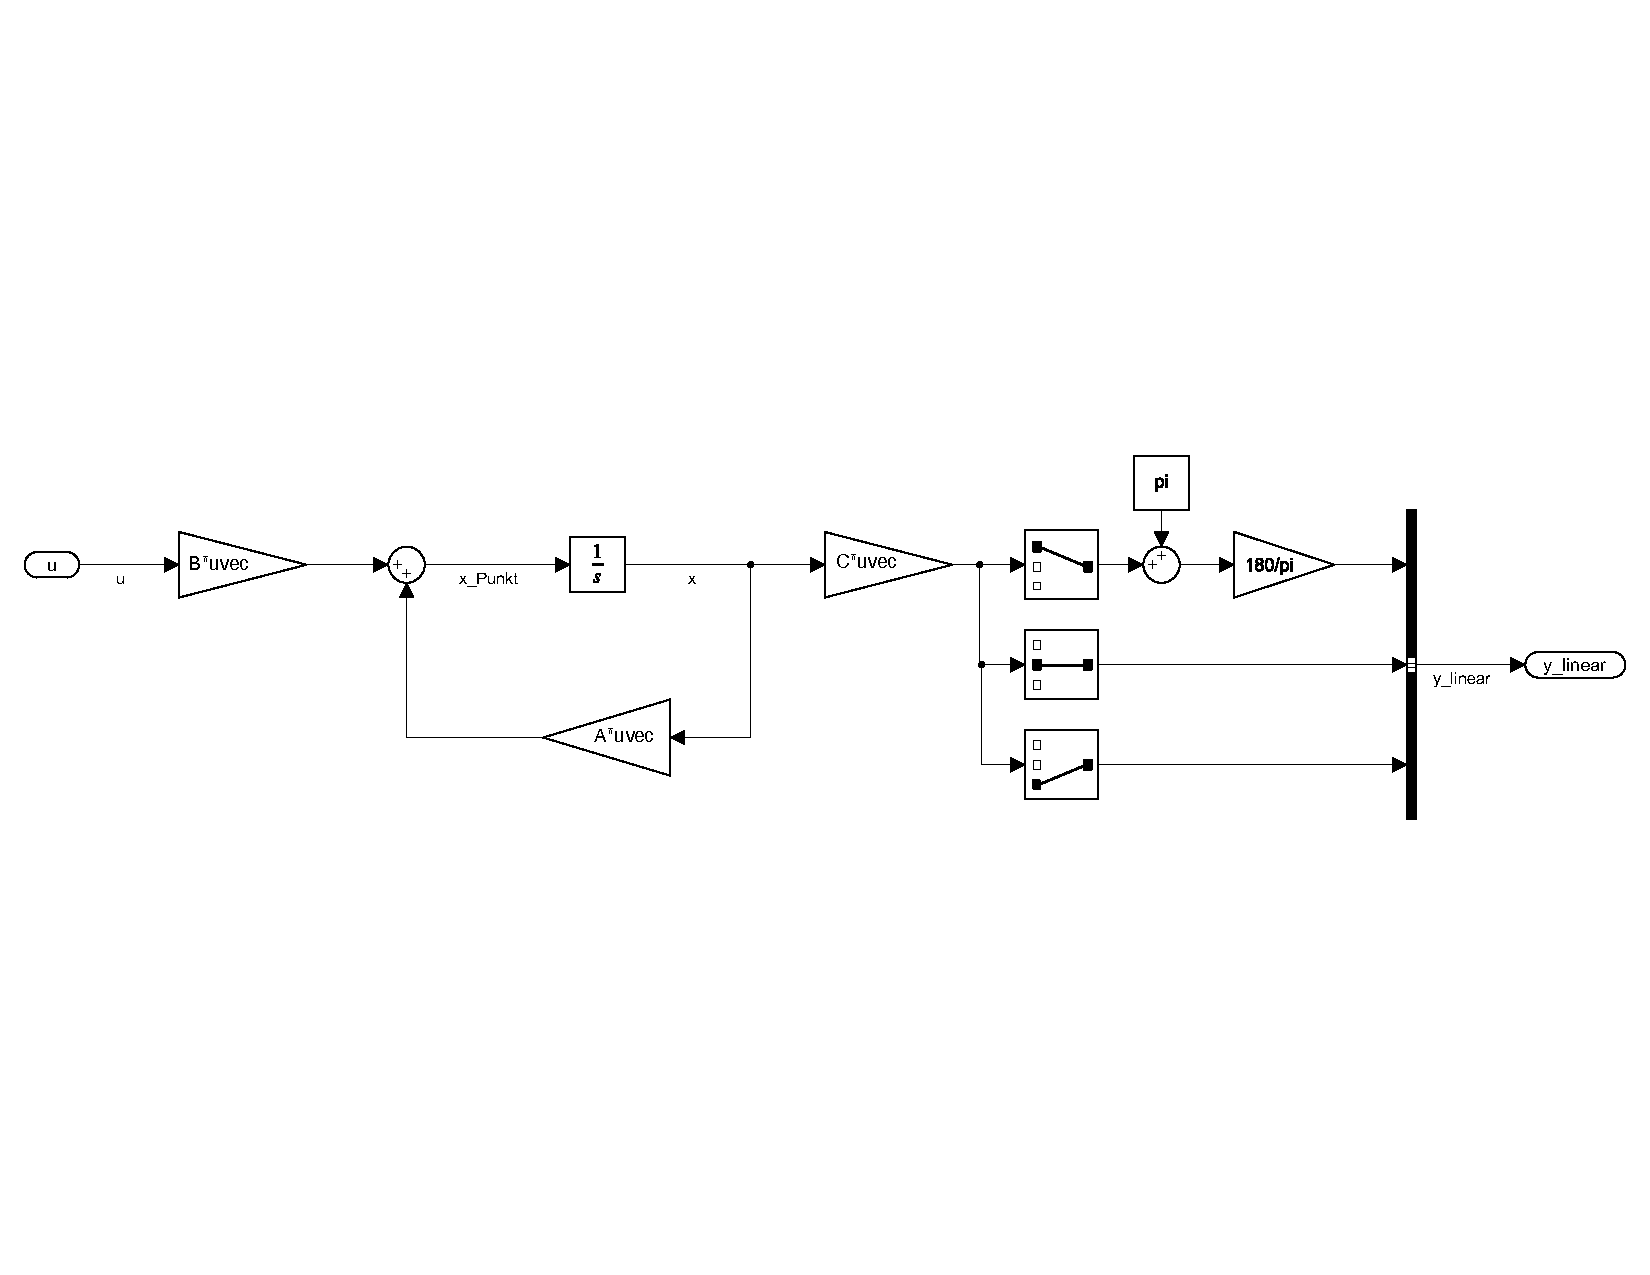
\includegraphics[width=0.85\textwidth]{Bilder/Lineare_Strecke.pdf}}
   \caption[Simulink-Modell des nichtlinearen Systems]{Simulink-Modell des nichtlinearen Systems}
   \label{fig:Bild2}
\end{figure}

\begin{figure}[H]
   \centering
   \fbox{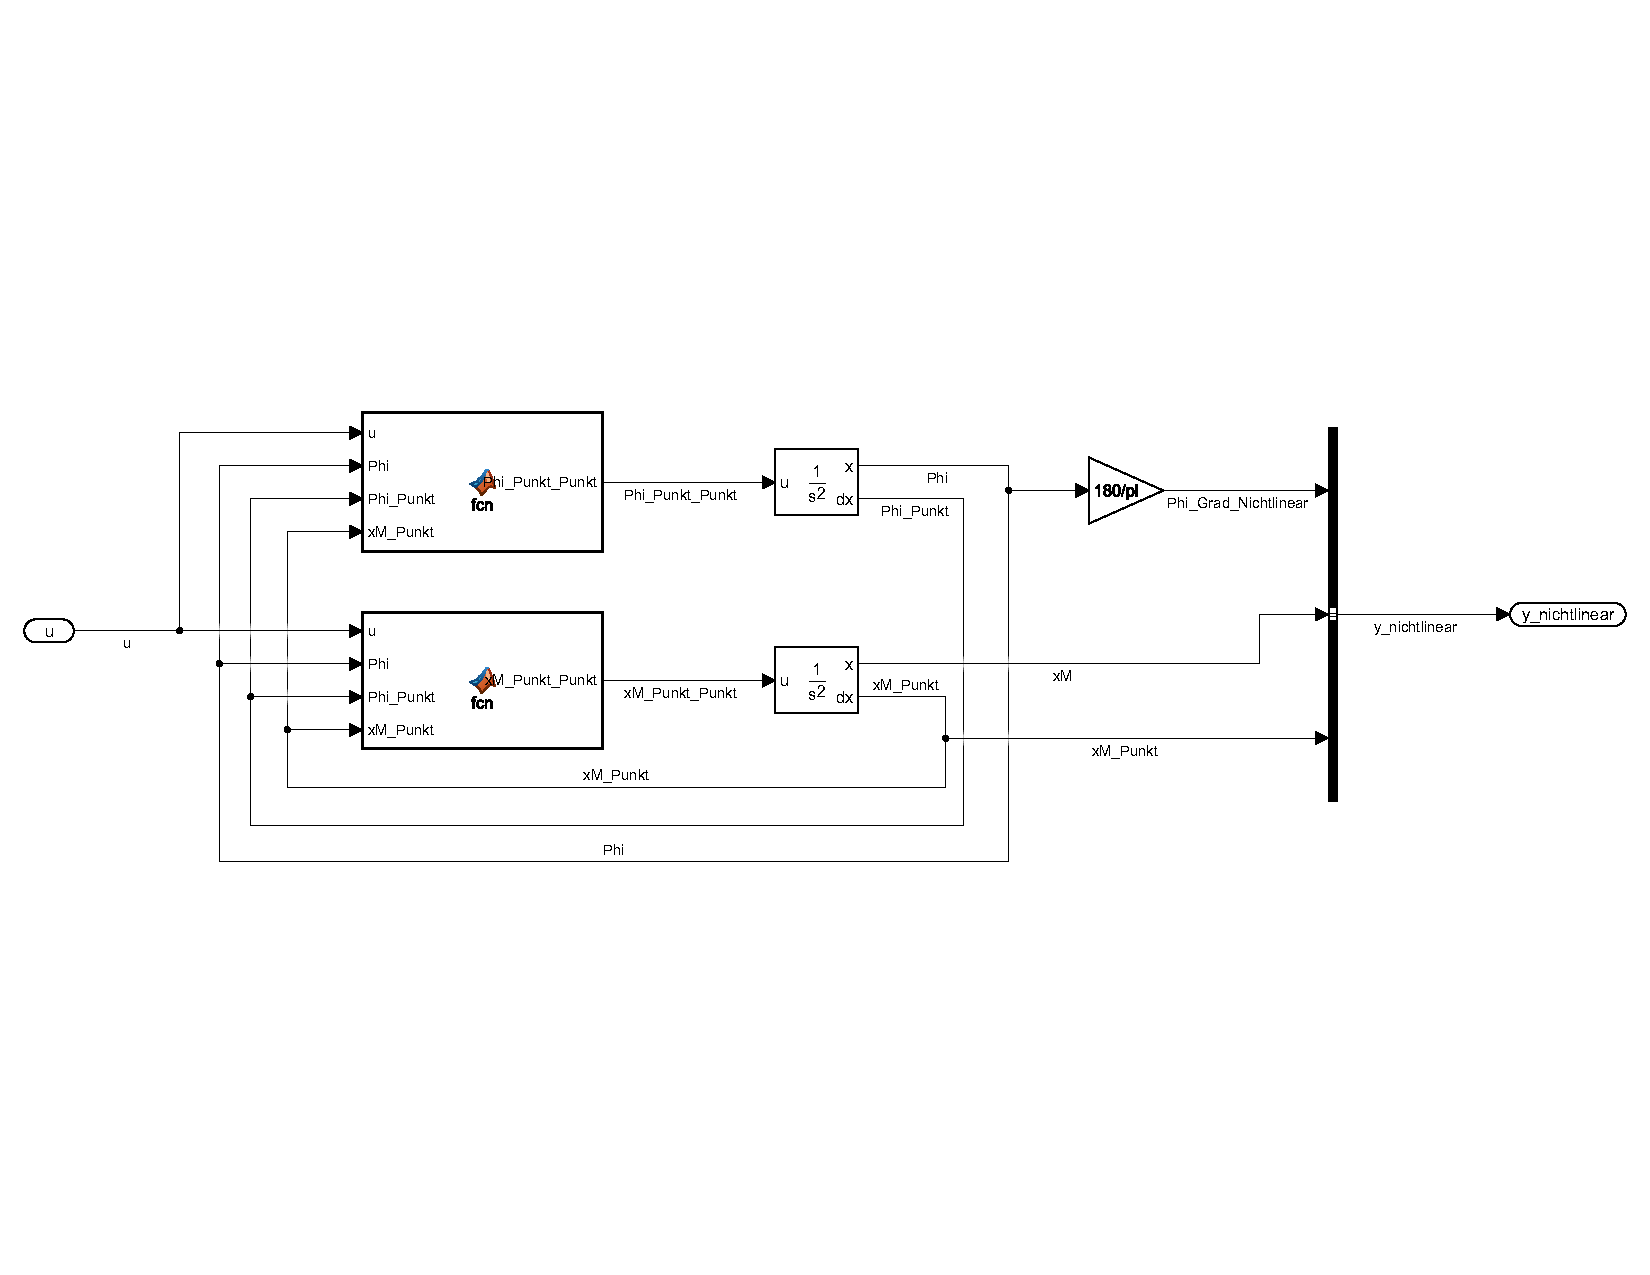
\includegraphics[width=0.85\textwidth]{Bilder/Nichtlineare_Strecke.pdf}}
   \caption[Simulink-Modell des linearisierten Systems]{Simulink-Modell des linearisierten Systems}
   \label{fig:Bild3}
\end{figure}

Beim Vergleich der beiden Systemverhalten ist zu erkennen, dass diese für kleine Winkelauslenkungen nahezu identisch erscheinen (\autoref{fig:Bild4} und \autoref{fig:Bild5}). Durch den sinusoidalen Signalverlauf wird weiter geschlussfolgert, dass eine positive Eingangskraft (Wagen fährt nach rechts) das Pendel in positive Winkelrichtung ausschlagen lässt. Da keine weiteren äußeren Kräfte auf das System eingeprägt werden, erfolgt mit steigender Zeit t durch die Reib- und Dämpfungsmomente das erneute Einpendeln in die stabile Ruhelage (hängendes Pendel).

\begin{figure}[H]
   \centering
   \fbox{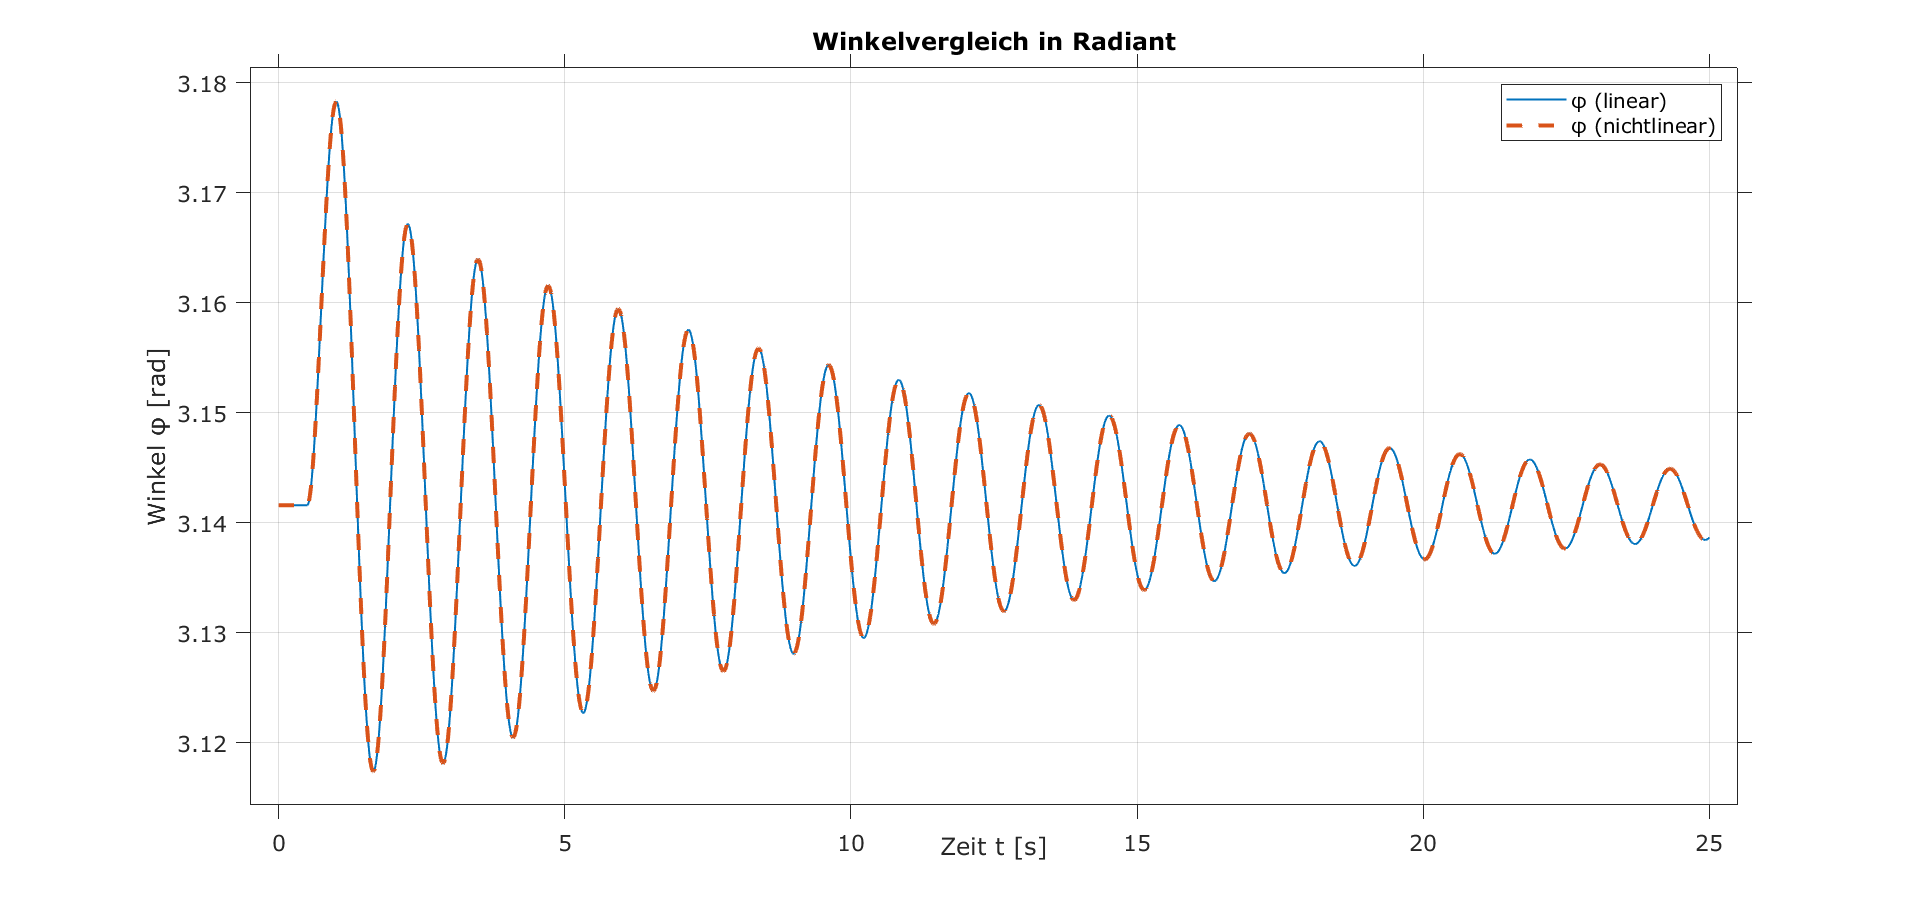
\includegraphics[width=0.9\textwidth]{Bilder/Phi_rad_Vergleich.png}}
   \caption[Vergleich der beiden radialen Winkelverläufe]{Vergleich der beiden radialen Winkelverläufe}
   \label{fig:Bild4}
\end{figure}

\begin{figure}[H]
    \centering
    \fbox{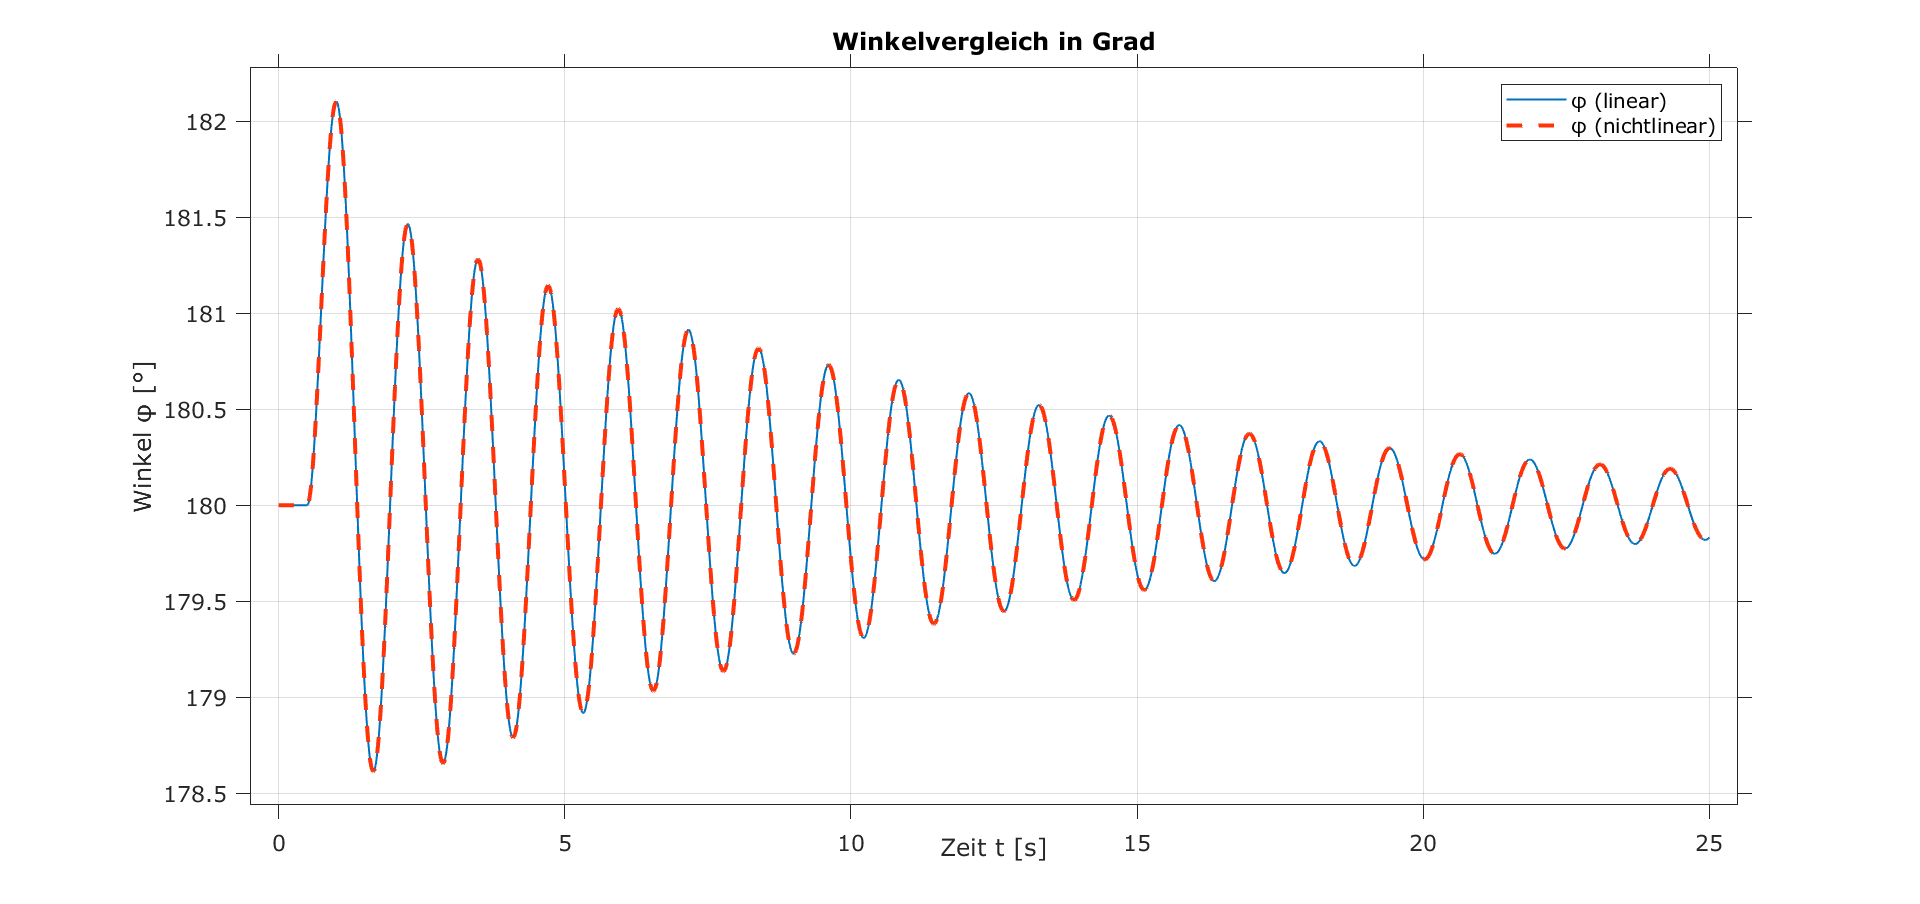
\includegraphics[width=0.9\textwidth]{Bilder/Phi_Grad_Vergleich.png}}
    \caption[Vergleich der beiden Winkelverläufe in Grad]{Vergleich der beiden Winkelverläufe in Grad}
    \label{fig:Bild5}
\end{figure}

Wird die Eingangskraft $F_{\mathrm{a}}$, welche auf das System wirkt, signifikant vergrößert (Einheitssprung mit Amplitude 15), werden größere Winkelauslenkungen erreicht. Dies führt zur Verringerung der Zuverlässigkeit des linearisierten Systems und zu Abweichungen zwischen dem linearen und nichtlinearem Systemverhalten (\autoref{fig:Bild6}).

\begin{figure}[H]
    \centering
    \fbox{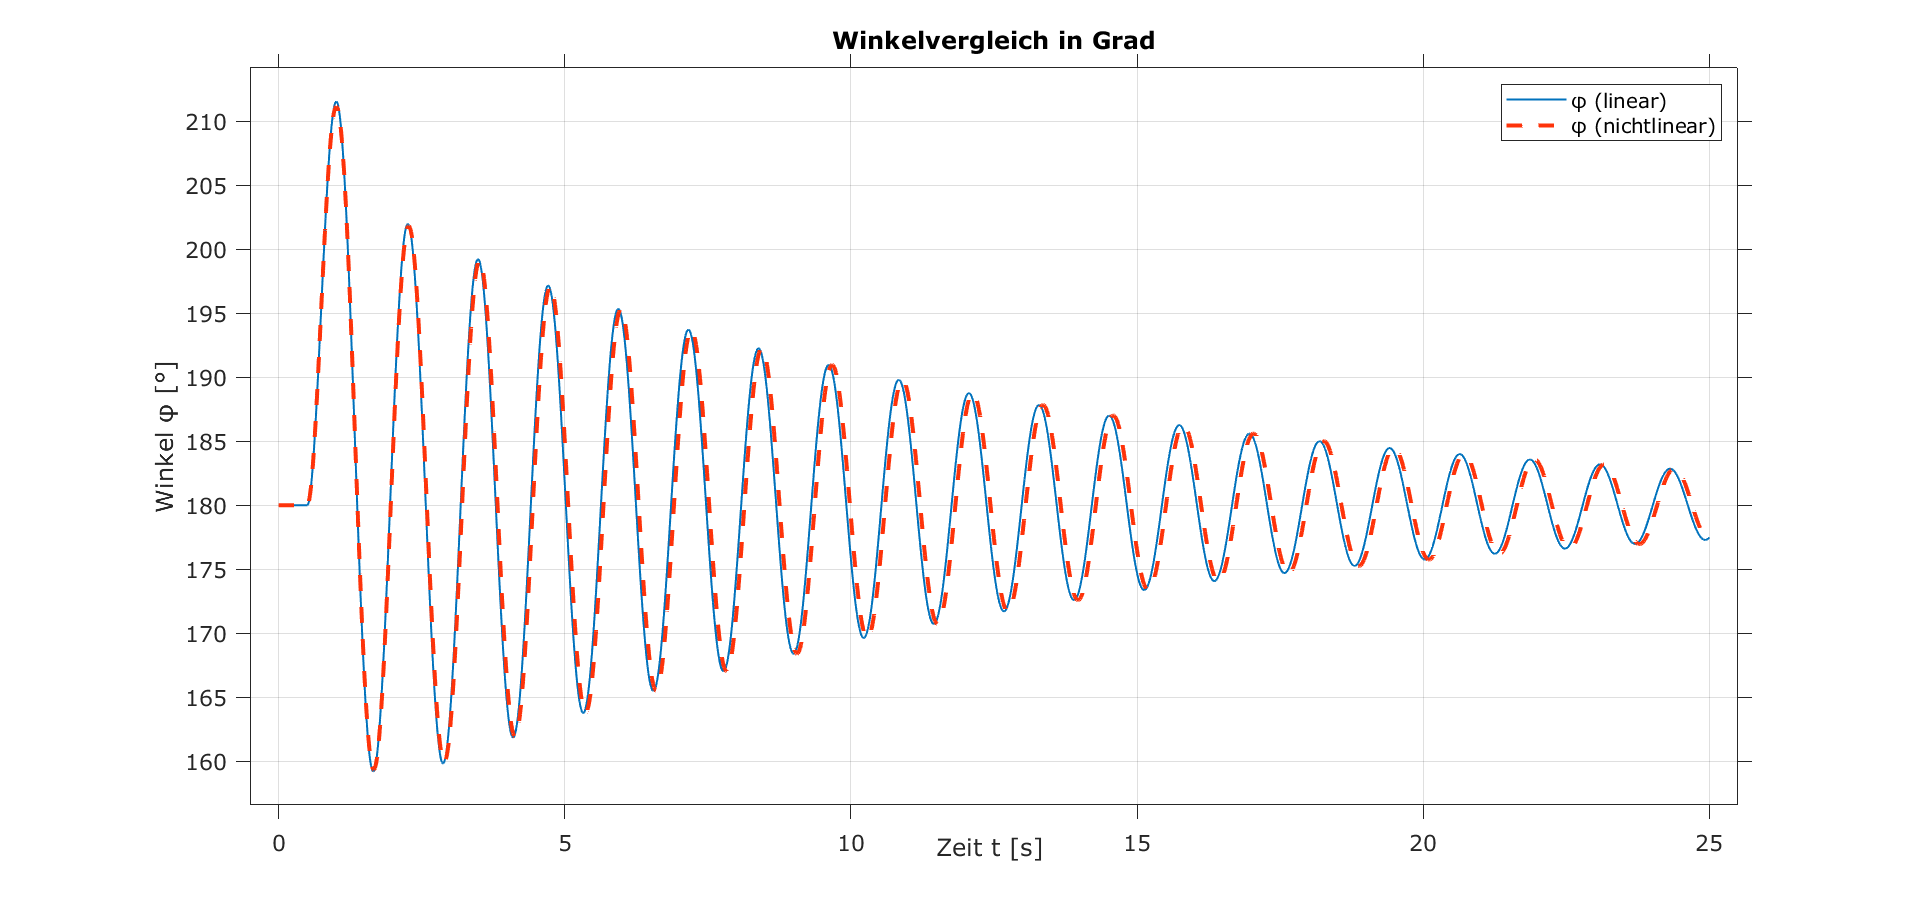
\includegraphics[width=0.9\textwidth]{Bilder/Phi_Grad_Vergleich_Verschiebung.png}}
    \caption[Vergleich der beiden Winkelverläufe in Grad mit Abweichung]{Abweichungen im Systemverhalten für größere Winkelauslenkungen}
    \label{fig:Bild6}
\end{figure}